\chapter{Methods}
\label{chap-methods}


\section{Disturbance models}

\subsection{Randomly-occurring deterministic disturbances}\label{subsec-RODD}

\textit{Randomly-occurring deterministic disturbances} (RODDs) \citep{macgregor_duality_1984} are a family of stochastic process models suitable for simulating various types of infrequently-occurring disturbances in discrete-time.  The structure of the RODD model is
\begin{equation} \label{eq:RODD}
	p(k)= \frac{B(q^{-1})}{A(q^{-1})}w_p(k),
\end{equation}
where $p(k)$ is the generated disturbance signal, $A(q^{-1})$ and $B(q^{-1})$ are arbitrary polynomial functions of the backward shift operator, $q^{-1}$, and $w_p(k)$ is a random variable generated by a switching system.

To generate randomly-occurring disturbances, the switching system,
\begin{equation} \label{eq:wpk1}
w_p(k) \sim 
\begin{cases*}
	0 & with probability $1-\epsilon$, \\
	\mathcal{N}\left(0, \sigma_{w_p}\right) & with probability $\epsilon$,
\end{cases*}
\end{equation}
may be used, where $w_p(k)$ is either 0 or is sampled from a normal distribution.  When the probability $\epsilon$ is low ($\epsilon<<1$), this system produces \textit{infrequent shocks}.

Alternatively, a mixture of two distributions may be used \citep{robertson_detection_1995}:
\begin{equation} \label{eq:wpk2}
w_p(k) \sim 
	\begin{cases*}
		\mathcal{N}\left(0, \sigma_{w_p}^2\right) & with probability $1-\epsilon$, \\
		\mathcal{N}\left(0, b^2\sigma_{w_p}^2\right) & with probability $\epsilon$.
	\end{cases*}
\end{equation}

In this formulation, $\sigma_{w_p}$ represents the standard deviation of the noise in periods between random shocks and $b$ is typically large so that the magnitude of the shocks is many times greater than $\sigma_{w_p}$. One benefit of (\ref{eq:wpk2}) is that the distribution of $w_p(k)$ is conditionally Gaussian, whereas in (\ref{eq:wpk1}) it has a non-smooth (i.e. degenerate) probability density function.

Figure \ref{fig:wpk-pdf} illustrates the probability density of $w_p(k)$ in the case of (\ref{eq:wpk2}) with $\sigma_{w_p}=0.01$, $b=100$, and $\epsilon=0.01$. Although it is difficult to discern from the plot, this is a mixture distribution with two components. The component that generates the infrequent shocks is barely visible because of its low probability. In this example, 99 percent of the probability lies within a narrow range (-0.036 < $w_p(k)$ < 0.036). However, the shocks, which occur with probability 0.01, have much higher amplitude ($b\sigma_{w_p}=1$).

\begin{figure}[htp]
	\centering
	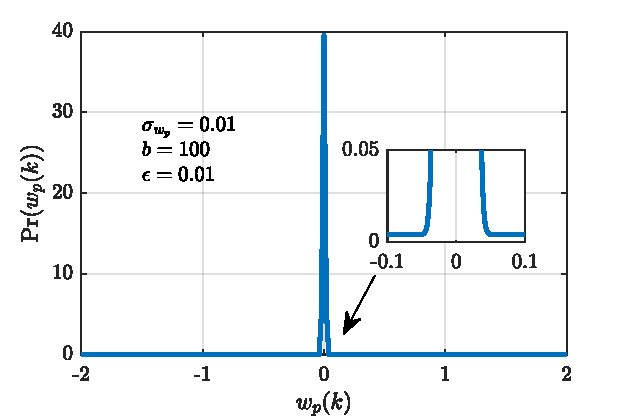
\includegraphics[width=11.5cm]{wpk-pdf-4.pdf}
	\caption{Probability density of a random shock signal}
	\label{fig:wpk-pdf}
\end{figure}

When dealing with a system having more than one RODD, where each random shock is independent, the notation is
\begin{equation} \label{eq:wpik2}
	w_{p,i}(k) \sim 
	\begin{cases*}
		\mathcal{N}\left(0, \sigma_{w_p,i}^2\right) & with probability $1-\epsilon_i$, \\
		\mathcal{N}\left(0, b_i^2\sigma_{w_p,i}^2\right) & with probability $\epsilon_i$.
	\end{cases*},
\end{equation}
where $i \in \left\{1, 2, ..., n_p\right\}$.

The choice of $A(q^{-1})$ and $B(q^{-1})$ in (\ref{eq:RODD}) determines the nature of the RODD. For example, if $B(q^{-1})=1$ and $A(q^{-1})=1-q^{-1}$, $p(k)$ will be a random-walk process with infrequent, large step changes.

Denoting $\nabla=1-q^{-1}$, the RODD \textit{step-disturbance} process can be defined as
\begin{equation} \label{eq:RODD-step}
	p(k)= \frac{1}{\nabla}w_p(k)
\end{equation}

A RODD \textit{ramp-disturbance}, consisting of a series of ramps with randomly-occurring changes in slope, may be generated using
\begin{equation} \label{eq:RODD-ramp}
	p(k)= \frac{1}{\nabla^2}w_p(k).
\end{equation}

A RODD consisting of randomly-occurring decaying exponential changes may be generated using
\begin{equation} \label{eq:RODD-exp}
	p(k)= \frac{1}{(1-a_1q^{-1})\nabla}w_p(k),
\end{equation}
where  $0<a_1<1$.

A disturbance with a combination of different RODD types is also possible.  For example, a state-space representation of a RODD combining step changes and ramps is

\begin{equation} \label{eq:RODD-step-ramp}
	\begin{split}
		\mathbf{x}_p(k+1) & =\left[\begin{array}{cc}
			1 & 1 \\
			0 & 1
		\end{array}\right] \mathbf{x}_p(k) +\left[\begin{array}{cc}
			1 & 0 \\
			0 & 1
		\end{array}\right] \mathbf{w}_p(k) \\
		p(k) & =\left[\begin{array}{cc}
			1 & 0
		\end{array}\right] \mathbf{x}_p(k),
	\end{split}
\end{equation}

where $\mathbf{x}_p(k) \in \mathbb{R}^2$ is a state vector and $\mathbf{w}_p(k)$ is a vector of two independent random shock signals generated by (\ref{eq:wpk1}), with possibly different parameter values. Simulated examples of these RODDs are presented in figures \ref{fig:rodd-sim-plots} and \ref{fig:rodd-sim-plot2} in section \ref{chap-simulation}.

\subsection{Hidden Markov Models}

\textit{Hidden Markov models} (HMM) can be used to simulate a more diverse set of switching behaviours than those of the RODD model described in the previous section \citep{wong_realistic_2009}. A Markov process or Markov chain is a stochastic model used to describe a sequence of discrete events in which the probability of future events depends only on the current state. A HMM is a Markov model with states that are not fully observable (i.e. hidden or observed with a measurement error).

To illustrate the basic concept, we can define the state of the random shock generating process (\ref{eq:wpk2}) as a Markov model state $\gamma(k)$ with two possible values:
\begin{equation} \label{eq:gamma-k}
	\gamma(k) = 
	\begin{cases*}
		0: & no shock, \\
		1: & shock.
	\end{cases*}
\end{equation}

$\gamma(k)=0$ represents the state of the process when no shock occurs and $\gamma(k)=1$ represents the state when a shock occurs.

The switching of $\gamma(k)$ can then be defined by a \textit{transition matrix}, $\Pi$, which describes the probabilities of transitioning from the state at time $k$ to the state at time $k+1$:
\begin{equation} \label{eq:Pi}
	\begin{split}
	\Pi = \left(\pi_{ij} \forall i,j\in \{1,2,...,n_j\}\right) \\
	\pi_{ij}=\Pr\left(\gamma(k)=j|\gamma(k-1)=i\right).
	\end{split}
\end{equation}

For example, to simulate the random shock signal used in the RODD model (\ref{eq:wpk2}), the transition probability matrix
\begin{equation} \label{eq:Pi-RODD-step}
	\Pi_{w_{p}} = \begin{bmatrix}
	1-\epsilon & \epsilon \\
	1-\epsilon & \epsilon
	\end{bmatrix}
\end{equation}
is used. In this case, since $w_{p}(k)$ is an independent random variable, it does not depend on the previous state. Therefore, the rows of $\Pi_{w_{p}}$ are identical.

The use of the Markov model thus allows transition probabilities that depend on the current state. For example, consider a disturbance where the signal switches infrequently between samples from two or more distributions with different parameters. The probabilities of switching from one distribution to another may be different. Such a disturbance process could be simulated with a hidden Markov model by conditioning the distribution from which $w_p(k)$ is sampled on the Markov state $\gamma(k)$:
\begin{equation} \label{eq:mog-example}
	\begin{split}
		w_p(k) \sim 
		\begin{cases*}
			\mathcal{N}\left(\mu_{w_p,1}, \sigma_{w_p,1}\right) & if $\gamma(k)=0$, \\
			\mathcal{N}\left(\mu_{w_p,2}, \sigma_{w_p,2}\right) & if $\gamma(k)=1$, \\
			... & ...\\
			\mathcal{N}\left(\mu_{w_p,n_j}, \sigma_{w_p,n_j}\right) & if $\gamma(k)=n_j-1$.
		\end{cases*} \\
	\Pr(\gamma(k)=j|\gamma(k-1)=i)=\pi_{ij} \forall i,j \in {1,2,...,n_j}
	\end{split}
\end{equation}

To make the notation more concise, allow the value of a time-varying discrete variable such as $\sigma_{w_p} \in \left\{\sigma_{w_p,1}, \sigma_{w_p,2},..., \sigma_{w_p,n_j}\right\}$, be determined by the value of the Markov state $\gamma(k)$. Thus,
\begin{equation} \label{eq:A-selection}
	\sigma_{w_p}(\gamma(k)) = 
	\begin{cases*}
		\sigma_{w_p,1} & if $\gamma(k)=0$, \\
		\sigma_{w_p,2} & if $\gamma(k)=1$, \\
		... & ...\\
		\sigma_{w_p,n_j} & if $\gamma(k)=n_j-1$.
	\end{cases*}
\end{equation}


With this notation, (\ref{eq:mog-example}) can be written more concisely as
\begin{equation} \label{eq:mog-example2}
	\begin{split}
		w_p(k) \sim \mathcal{N}\left(\mu_{w_p}(\gamma(k)), \sigma_{w_p}(\gamma(k))\right) \\
		\Pr(\gamma(k)=j|\gamma(k-1)=i)=\pi_{ij} \forall i,j \in {1,2,...,n_j}.
	\end{split}
\end{equation}
where $\mu_{w_p}\in\left\{\mu_{w_p,1},\mu_{w_p,2},...,\mu_{w_p,n_j}\right\}$. This model is known as a \textit{mixture of Gaussians} and can be considered a special-case of a HMM-based disturbance model \citep{wong_disturbance_2007}.

The general HMM disturbance process is described by the following \textit{Markov jump linear system} (MJLS) \citep{costa_discrete-time_2005}. This is a state-space representation with time-varying system matrices $\mathbf{A}(\gamma(k))$, $\mathbf{B}(\gamma(k))$, and $\mathbf{C}(\gamma(k))$:
\begin{equation} \label{eq:HMM}
	\begin{split}
	\mathbf{x}_p(k+1) = \mathbf{A}(\gamma(k))x_p(k) + \mathbf{B}(\gamma(k))\mathbf{w}_p(k) \\
	\mathbf{p}(k) = \mathbf{C}(\gamma(k)) \mathbf{x}_p(k) + \mathbf{e}_p(k)
	\end{split}
\end{equation}

As well as $\mathbf{w}_p(k)$, $\mathbf{e}_p(k)$ may also be a switching random variable. This is a versatile dynamic model suitable for representing and simulating a diverse family of disturbances.

\subsection{Bounded disturbances}

The \textit{bounded random walk} (BRW) is a stochastic process proposed by \citep{nicolau_stationary_2002}. The discrete-time version has the difference equation

\begin{equation} \label{eq:brw}
		p(k+1) = p(k) + a(p(k)) + e(k)
\end{equation}

where $e(k)$ is a random noise with variance $\sigma_e^2$, and $a(p(k))$ is a function defined as

\begin{equation}
	a(x) = e^{\beta}\left(e^{-\alpha_{1}\left(x - \tau\right)} - e^{\alpha_{2}\left(x - \tau\right)}\right)
\end{equation}

where $\beta$, $\alpha_{1}$, and $\alpha_{2}$ are constants.  From (\ref{eq:brw}) it can be deduced that

\begin{equation}
	E(p(k+1)|p(k)) = p(k) + a(p(k)).
\end{equation}

Therefore $a(p(k))$ has the effect of an additive bias or adjustment to $p(k+1)$ which depends on $p(k)$. The shape of $a(x)$ depends on the constants. Figure \ref{fig:brw-a} shows $a(x)$ in the case where $\tau=100$, $\beta=-15$, $\alpha_{1}=3$, and $\alpha_{2}=3$.  From this, it is clear that in the vicinity of $x=\tau$, $a(x)\approx0$. When $a(p(k))=0$, (\ref{eq:brw}) is the equation for a random walk. However, outside a certain neighbourhood around $x=\tau$, $a(x)$ increases for low $x$ or decreases for high $x$. This has the effect of causing $p(k+1)$ to revert towards the mean ($\tau$) whenever $p(k)$ strays outside the neighbourhood. 

\begin{figure}[htp]
	\centering
	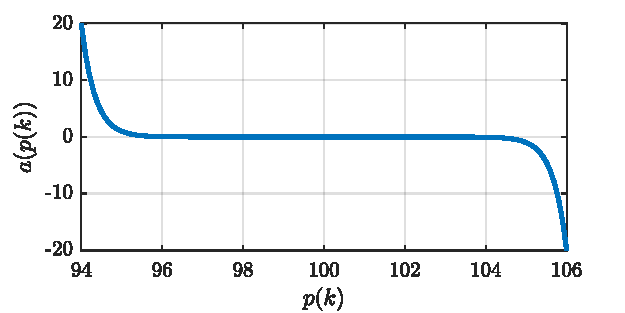
\includegraphics[height=5cm]{images/brw_a.pdf}
	\caption{A bounded random walk bias function}
	\label{fig:brw-a}
\end{figure}

Figure \ref{fig:brw-sim} shows a simulation of a bounded random walk with the parameter values as above, and for comparison, an unbounded random walk (labelled `RW') generated with the same noise input. The dashed lines at $p(k)=95$ and $p(k)=105$ roughly indicate the location of the lower and upper bounds which the BRW only marginally exceeds.

\begin{figure}[htp]
	\centering
	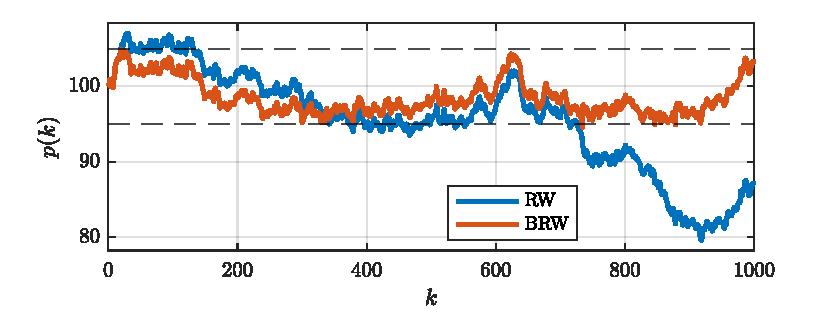
\includegraphics[height=5cm]{images/brw_sim.pdf}
	\caption{Examples of a bounded and unbounded random walk}
	\label{fig:brw-sim}
\end{figure}

Unlike a simple random walk, the BRW is stationary. \cite{nicolau_stationary_2002} derived a formula for the form of the unconditional probability distribution of the continuous-time BRW. Figure \ref{fig:brw-pdf} shows the normalized stationary probability density with the same parameter values as above. For comparison, the probability density of a random walk process after 20 sample periods is also shown. It can be seen that there is a significant probability that the random walk would exceed the bounds of this BRW after 20 sample periods. It can also be seen that the central part of the probability distribution of the BRW is flat, indicating that all values within the bounds are equally likely after a large number of samples, similar to a uniform probability distribution.

%\begin{equation}
%	p_{BRW}(x) \propto \sigma^{-2} \exp \left\{-\frac{2 e^{k}}{\sigma^{2}}\left(\frac{e^{-\alpha_{1}(x-\tau)}}{\alpha_{1}}+\frac{e^{\alpha_{2}(x-\tau)}}{\alpha_{2}}\right)\right\}
%\end{equation}

\begin{figure}[htp]
	\centering
	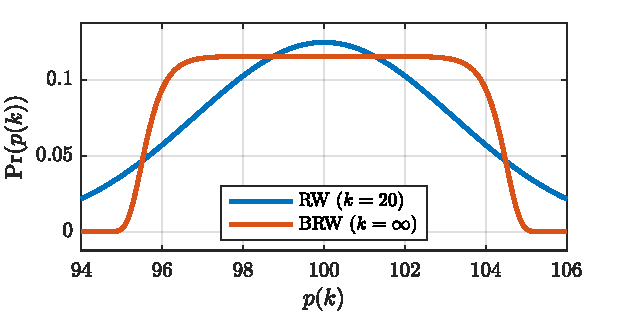
\includegraphics[height=5cm]{images/brw_pdf.pdf}
	\caption{Probability distributions of bounded and unbounded random walks}
	\label{fig:brw-pdf}
\end{figure}

However, the BRW as described by (\ref{eq:brw}) is not guaranteed to be stable.  For extreme values of $p(k)$, $|a(p(k))|$ may be greater than $2|p(k)|$.  This means that $|p(k)|$ will increase rapidly, leading to numerical errors in any practical implementation.  To avoid this, \cite{nicolau_stationary_2002} recommends adding a conditional regularizing step which causes reversion towards the mean, $\tau$, when the correction bias is too large. Instead of (\ref{eq:brw}), the conditional difference equation
\begin{equation} \label{eq:brw-reg}
	p(k+1) = \begin{cases*}
		p(k) + a(p(k)) + e(k) & if $\left|a(p(k)) \right| < 2\left| p(k) - \tau \right|$, \\
		\tau + \phi(p(k) - \tau) + e(k) & if $\left|a(p(k)) \right| \geq 2\left| p(k) - \tau \right|$
	\end{cases*}
\end{equation}
is used, where $\phi$ is a constant such that $0<\phi<1$. The size of $\phi$ determines how fast $p(k)$ reverts to $\tau$, the stationary mean of the BRW, when it is outside the stable region.

Since the BRW has a non-Gaussian probability distribution, analysis of the properties of any dynamical system with a BRW input is difficult. However, for simulation purposes, the BRW is a simple and practical solution to the problem of bounding a random variable.

The BRW concept can easily be extended to RODDs. For example, a RODD step disturbance (\ref{eq:RODD-step}) is a random walk with a switching noise variance (\ref{eq:wpk2}). The concern when trying to bound this disturbance is the large step change that occurs infrequently. Since the probability of the shock, as well as the sign and amplitude of the step, are independent random variables, a RODD step disturbance that happens to be at one of the bounds is as likely to step outside the bound as it is to step back inside the bounded region. Therefore, the conditional regularity used in the BRW (\ref{eq:brw-reg}) is even more important.


\section{State estimation}

State estimation is the task of estimating the values of the state variables of a dynamic model of a system given a set of measurements from the system. In process control applications, state estimates are required online (i.e. in real time), in order to provide the best possible estimate of the states at the current time (or a prediction of their values at the next time instant) in order to calculate an appropriate control action.

Consider the diagram of an input-output system model in Figure \ref{fig:model_diag_uwvy}. Here, $\mathbf{u}(k) \in \mathbb{R}^{n_u}$ is a vector of measured input variables at time instant $k$, $\mathbf{w}(k) \in \mathbb{R}^n$ is a vector of unmeasured state disturbances, $\mathbf{v}(k) \in \mathbb{R}^{n_y}$ is a vector of output disturbances or measurement errors, and $\mathbf{y}(k) \in \mathbb{R}^{n_y}$ is the vector of output variables. The box represents the mathematical model which relates the inputs to the outputs.

\begin{figure}[htp]
	\centering
	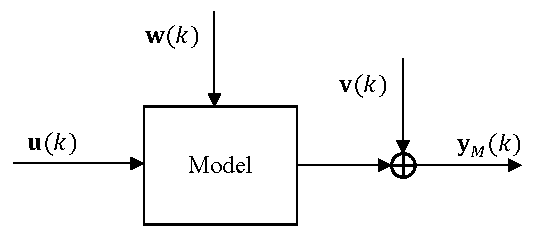
\includegraphics[width=8cm]{images/model_diag_uwvy.pdf}
	\caption{System model diagram}
	\label{fig:model_diag_uwvy}
\end{figure}

The most convenient form in which to represent discrete-time, linear, time-invariant, dynamical system models for state estimation and control purposes, is the state-space representation

\begin{equation} \label{eq:ss_rep_uwy}
	\begin{aligned}
		\mathbf{x}(k+1) = \mathbf{A} \mathbf{x}(k) + \mathbf{B} \mathbf{u}(k) + \mathbf{w}(k), \\
		\mathbf{y}(k) = \mathbf{C} \mathbf{x}(k) + \mathbf{v}(k).
	\end{aligned}
\end{equation}

where $\mathbf{x}(k) \in \mathbb{R}^n$ is a vector of state variables, $\mathbf{A} \in \mathbb{R}^{n \times n}$ is the state transition matrix, $\mathbf{B} \in \mathbb{R}^{n \times n_u}$ is the input matrix, $\mathbf{C} \in \mathbb{R}^{n_y \times n}$ is the output matrix.

\begin{figure}[htp]
	\centering
	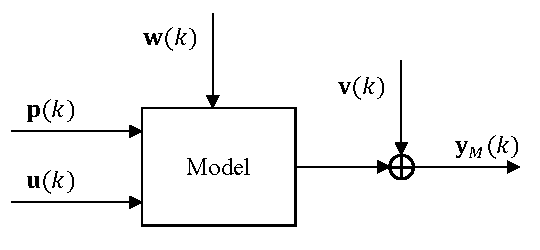
\includegraphics[width=8cm]{images/model_diag_upwvy.pdf}
	\caption{System model with disturbance inputs and manipulatable inputs}
	\label{fig:model_diag_upwvy}
\end{figure}

The \textit{Kalman filter} \citep{kalman_new_1961} is the optimal estimator for a linear system in which the unmeasured disturbances and measurement errors are Gaussian random variables. The predictions of the states at the next time instant, $k+1$, calculated at the current time $k$, are given by
\begin{equation} \label{eq:xkp1_hat}
	\mathbf{\hat{x}}(k+1/k) = \mathbf{A} \mathbf{\hat{x}}(k/k-1) + \mathbf{B}\mathbf{u}(k) + 
	\mathbf{K}(k)\left[\mathbf{y}(k) - \mathbf{C} \mathbf{\hat{x}}(k/k-1)\right],
\end{equation}
where $\mathbf{\hat{x}}(k/k-1)$ is the previous prediction of the states at the current time, calculated in the previous time instant, $\mathbf{y}(k)$ is the current measurement of the output, and $\mathbf{K}(k) \in \mathbb{R}^{n \times n_y}$ is a correction gain matrix. An intuitive interpretation of the Kalman filter is that it iteratively updates the state estimates based on the difference between the output predicted by the system model, $\mathbf{C} \mathbf{\hat{x}}(k/k-1)$, and the output measurement ${y}(k)$.

In the case of a steady-state Kalman filter, $\mathbf{K}(k)$ is constant (time-invariant). However, in general, it is calculated at each time step using
\begin{equation} \label{eq:Kk}
	K(k) = \mathbf{A}\mathbf{P}(k/k-1)\mathbf{C}^\intercal \big(\mathbf{C}\mathbf{P}(k/k-1)\mathbf{C}^\intercal + \mathbf{R}\big)^{-1},
\end{equation}
where $\mathbf{P}(k/k-1)$ is the estimation error covariance matrix calculated in the previous time instant, and $\mathbf{R}$ is the covariance matrix of the measurement noises,
\begin{equation} \label{eq:R}
	\mathbf{R} = E\{ \mathbf{v}(k) \mathbf{v}^\intercal(k) \}.
\end{equation}

$\mathbf{P}(k/k-1)$ is updated every time step using
\begin{multline} \label{eq:Pk}
	\mathbf{P}(k+1/k) = \\ \mathbf{A}\big[\mathbf{P}(k/k-1)
	- \mathbf{P}(k/k-1)\mathbf{C}^\intercal\big(\mathbf{C}\mathbf{P}(k/k-1)\mathbf{C}^\intercal + 
	\mathbf{R}\big)^{-1}\mathbf{C}\mathbf{P}(k/k-1) \big]\mathbf{A}^\intercal + \mathbf{Q},
\end{multline}
where $\mathbf{Q}$ is the covariance matrix of estimation errors,
\begin{equation} \label{eq:Q}
	\mathbf{Q} = E\{ \mathbf{w}(k) \mathbf{w}^\intercal(k) \}.
\end{equation}

The state estimates, $\mathbf{\hat{x}}(k+1/k)$, are calculated recursively online, starting at time $k=0$, using (\ref{eq:xkp1_hat}), (\ref{eq:Kk}) and (\ref{eq:Pk}), provided that initial values of the state estimates, $\mathbf{\hat{x}}(0)$, and estimation error covariance matrix $\mathbf{P}(0)$, are available.

In the case where the system has additional disturbance inputs, $\mathbf{p}(k) \in \mathbb{R}^{n_p}$, as shown in Figure \ref{fig:model_diag_upwvy}, the state-space equations are modified to include these and the input matrix is split into two, $\mathbf{B}_u \in \mathbb{R}^{n \times n_u}$ and $\mathbf{B}_p \in \mathbb{R}^{n \times n_p}$,
\begin{equation} \label{eq:ss_rep_upwy}
	\begin{aligned}
		\mathbf{x}(k+1) = \mathbf{A} \mathbf{x}(k) + \mathbf{B}_u \mathbf{u}(k) + \mathbf{B}_p \mathbf{p}(k) + \mathbf{w}(k), \\
		\mathbf{y}(k) = \mathbf{C} \mathbf{x}(k) + \mathbf{v}(k).
	\end{aligned}
\end{equation}

For state estimation in the presence of disturbances, which is always the case in practice, a suitable model of the disturbances is needed. This additional model is shown in Figure \ref{fig:model_diag_wpupwvy} with an additional set of random variables $\mathbf{w}_p(k)$ at its input.

\begin{figure}[htp]
	\centering
	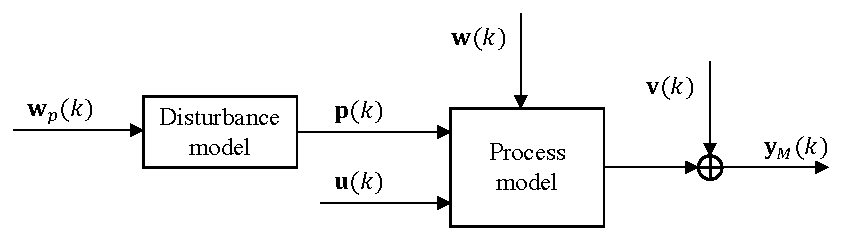
\includegraphics[width=12.5cm]{images/model_diag_wpupwvy.pdf}
	\caption{System with process model and disturbance model}
	\label{fig:model_diag_wpupwvy}
\end{figure}

A state-space representation of the combined system including the disturbance model can be constructed. This will be referred to as the \textit{augmented model},
\begin{equation} \label{eq:ss_rep_xa}
	\begin{aligned}
		\mathbf{x}_a(k+1) = \mathbf{A}_a \mathbf{x}_a(k) + \mathbf{B}_{a,u} \mathbf{u}(k) + \mathbf{B}_{a,w} \mathbf{w}_{a}(k), \\
		\mathbf{y}(k) = \mathbf{C}_a \mathbf{x}_a(k) + \mathbf{v}(k),
	\end{aligned}
\end{equation}
where $\mathbf{x}_a(k) \in \mathbb{R}^{n+n_p}$ is an augmented state vector which includes the states of both the process model and the disturbance model, and $\mathbf{w}_a(k) \in \mathbb{R}^{n+n_p}$ is an augmented vector of random variables (i.e. $\mathbf{w}(k)$ and $\mathbf{w}_p(k)$ combined).


\subsection{Multiple model approaches}

Although the random shock in a RODD is unmeasured, it may be observable from the measurements of the outputs of the system. However, as mentioned in Section \ref{chap-lit-review}, systems with RODDs pose problems for state estimation using standard Kalman filters due to the switching of the noise model parameters, namely, the variance of $w_p(k)$ (\ref{eq:wpk2}). As explained by \cite{robertson_detection_1995}, a trade-off must be made during the filter design between its ability to respond to the infrequent disturbance when it occurs, and its sensitivity to noise at other times.

Alternatively, a so-called \textit{multiple-model approach} may be considered \citep{buxbaum_recursive_1969, jaffer_estimation_1971}. Multi-model observers account for different possible hypotheses about the current and past states of the system and infer from these an overall `best' estimate of the current states. To achieve this, an independent Kalman filter is maintained for each hypothesis and a weighted average of the estimates by each filter is calculated using the conditional probabilities of each hypothesis given current and past measurements.

Let the number of Kalman filters be $n_f$ and the \textit{shock occurrence hypothesis} associated with Kalman filter $f$ at time instant $k$ be
\begin{equation} \label{eq:gammak}
	\gamma_{f}(k) \in \left\{0, 1 \right\} \forall{k \ge 0}.
\end{equation}

First, consider the case of estimating only one shock signal (\ref{eq:wpk2}). Therefore, $\gamma_{f}(k)$ is a scalar. The transition probabilities of the random shock are independent of previous shocks:
\begin{equation} \label{eq:Pr_gammak_given_gammakm1}
	\begin{aligned}
		& \Pr\left(\gamma_{f}(k)=0 \mid \gamma_{f}(k-1)\right) = 1-\epsilon, \\
		& \Pr\left(\gamma_{f}(k)=1 \mid \gamma_{f}(k-1)\right) = \epsilon.
	\end{aligned}
\end{equation}

After $k$ time steps, the complete shock occurrence hypothesis associated with filter $f$ is
\begin{equation} \label{eq:Gammak}
	\Gamma_f(k) = \left\{\gamma_f(0), \gamma_f(1), ..., \gamma_f(k) \right\}.
\end{equation}

The measurements up to time $k$ are
\begin{equation} \label{eq:Uk_Yk}
	\begin{aligned}
		\mathbf{U}(k)=\left\{\mathbf{u}(0), \mathbf{u}(1), ..., \mathbf{u}(k) \right\} \\
		\mathbf{Y}(k)=\left\{\mathbf{y}(0), \mathbf{y}(1), ..., \mathbf{y}(k) \right\}.
	\end{aligned}
\end{equation}

Assume that new measurement data is made available at each time instant. The probability of the shock sequence associated with filter $f$ given the data up to time $k-1$ can be calculated recursively:
\begin{multline} \label{eq:Pr_Gammakp1_given_Yk}
	\Pr(\Gamma_f(k) \mid \mathbf{Y}(k-1)) = 
	\Pr(\gamma_f(k) \mid \gamma_f(k-1)) \Pr(\Gamma_f(k-1) \mid \mathbf{Y}(k-1)).
\end{multline}
The conditional probability densities of the measurements $\mathbf{y}(k)$ are approximated by Gaussian distributions
\begin{equation} \label{eq:p_yk_given_Gammak_Ykm1}
	p(\mathbf{y(k)} \mid \Gamma_f(k), \mathbf{Y}(k-1)) \approx
	\mathcal{N}\left(\mathbf{y}(k), \mathbf{C} \mathbf{\hat{x}}_{f}(k/k-1), \mathbf{C} \mathbf{P}_f(k/k-1) \mathbf{C}^\intercal+\mathbf{R}\right)
\end{equation}
where $p(\cdot)$ here represents a probability density function, $\mathbf{\hat{x}}_{f}(k/k-1)$ and $\mathbf{P}_f(k/k-1)$ are the state estimates and estimate covariances of each Kalman filter at the previous time step, and $\mathcal{N}(\mathbf{y}, \mathbf{\mu}, \Sigma)$ is the multivariate normal probability density of $\mathbf{y}$ with mean $\mathbf{\mu}$ and variance $\Sigma$.

The estimate of the probability of the shock sequence $\Gamma_f(k)$ given the data up to time $k$ is
\begin{equation} \label{eq:Pr_Gammak_given_Yk}
	\Pr(\Gamma_f(k) \mid \mathbf{Y}(k)) = \frac{q_f(k)}{\sum_{f=1}^{n_f} q_f(k)},
\end{equation}
where
\begin{equation} \label{eq:qfk}
	q_f(k) = p(\mathbf{y}(k) \mid \Gamma_f(k), \mathbf{Y}(k-1)) \Pr(\Gamma_f(k) \mid \mathbf{Y}(k-1)).
\end{equation}

The Kalman filters for tracking each hypothesis use the state-space representation of the augmented system model (\ref{eq:ss_rep_xa}). 
However, in the case of a system with a RODD, the disturbance inputs include the non-Gaussian random variable, $\mathbf{w}_p(k)$, as well as the usual Gaussian disturbances on the rest of the states, $\mathbf{w}(k)$:
\begin{equation} \label{eq:wak}
	\mathbf{w}_a(k) = \begin{bmatrix}
		\mathbf{w}(k) \\
		\mathbf{w}_p(k)
	\end{bmatrix}.
\end{equation}

The system is therefore a \textit{hybrid dynamical system} because it has a switching noise covariance matrix. Define the set of possible covariance matrices as
\begin{equation} \label{eq:init_Q_R}
	\mathcal{Q} = \left\{\mathbf{Q}_0, \mathbf{Q}_1\right\},
\end{equation}

and, for convenient notation, let $\mathcal{Q}$ be indexed by the shock indicator variable $\gamma_f(k)$:
\begin{equation} \label{eq:init_Q}
	\mathcal{Q}(\gamma_f(k)) = 
	\begin{cases*}
		\mathbf{Q}_0 & \text{if} $\gamma_f(k)=0$, \\
		\mathbf{Q}_1 & \text{if} $\gamma_f(k)=1$.
	\end{cases*}
\end{equation}

At the start of simulation, filter $f$ has an initial estimate of the states, $\mathbf{\hat{x}}_f(0)$, and an initial estimate covariance $\mathbf{P}_f(0)$. At each time instant, starting at $k=0$, the filter correction gain is updated as in (\ref{eq:Kk})
\begin{equation} \label{eq:Kf}
	K_f(k) = \mathbf{A}\mathbf{P}_f(k/k-1)\mathbf{C}^\intercal \big(\mathbf{C}\mathbf{P}_f(k/k-1)\mathbf{C}^\intercal + \mathbf{R}\big)^{-1},
\end{equation}

the corrected state estimate at time $k+1$ is calculated as in \ref{eq:xkp1_hat}
\begin{equation} \label{eq:xfkp1_hat}
	\mathbf{\hat{x}}_f(k+1/k) = \mathbf{A} \mathbf{\hat{x}}_f(k/k-1) + \mathbf{B}\mathbf{u}(k) + 
	\mathbf{K}_f(k)\left[\mathbf{y}(k)-\mathbf{C} \mathbf{\hat{x}}_f(k/k-1)\right],
\end{equation}

and the estimation error covariance is updated using
\begin{multline} \label{eq:Pfk}
	\mathbf{P}_f(k+1/k) = \mathbf{A}\big[\mathbf{P}_f(k/k-1)
	- \mathbf{P}_f(k/k-1)\mathbf{C}^\intercal\big(\mathbf{C}\mathbf{P}_f(k/k-1)\mathbf{C}^\intercal \\ + 
	\mathbf{R}\big)^{-1}\mathbf{C}\mathbf{P}_f(k/k-1) \big]\mathbf{A}^\intercal + \mathcal{Q}(\gamma_f(k)). \\
\end{multline}

Note the difference between (\ref{eq:Pfk}) and (\ref{eq:Pk}).  Here, $\mathbf{P}_f(k+1/k)$ is dependent on $\gamma_f(k)$, which determines the noise covariance matrix used in the update, whereas in (\ref{eq:Pk}), $\mathbf{Q}$ is time invariant.

Finally, the multi-model observer estimate of the states in the next time instant is the sum of the $n_f$ Kalman filter estimates weighted by their conditional probabilities:
\begin{equation} \label{eq:x_hat}
	\mathbf{\hat{x}}(k+1/k) = \sum_{f=1}^{n_f} \mathbf{\hat{x}}_f(k+1/k) \Pr(\Gamma_f(k) \mid \mathbf{Y}(k))
\end{equation}

% TODO: in Robertson et al, they estimate x(k/k) not x(k+1/k).

Algorithm \ref{alg:afmm} is the iterative algorithm used to execute these computations.

\begin{algorithm}
	\caption{Multiple model observer calculations}  \label{alg:afmm}
	%\algorithmfootnote{$y_0$ denotes the initial value.}
	\begin{algorithmic}
			\Require $\mathbf{A},\mathbf{B},\mathbf{C},\mathbf{\hat{x}}(0), \mathbf{P}(0), \mathcal{Q}, \mathbf{R}, \epsilon, \mathbf{U}(N), \mathbf{Y}(N)$
			\State $\mathbf{\hat{x}}_1(0) \gets \mathbf{\hat{x}}(0)$  \Comment{Initialize Kalman filters}  % \footnotemark
			\State $\mathbf{P}_1(0) \gets \mathbf{P}(0)$
			\State $\Pr(\Gamma_1(k-1)|\mathbf{Y}(k-1))) \gets 1$
			\For{$f \gets 2, n_f$}
			\State $\mathbf{\hat{x}}_f(0) \gets \mathbf{\hat{x}}(0)$
			\State $\mathbf{P}_f(0) \gets 10^{10}\mathbf{P}(0)$
			\State $\Pr(\Gamma_f(k-1)|\mathbf{Y}(k-1))) \gets 1^{-10}$
			\EndFor
			\For{$k \gets 0, N$}
			\State $\Gamma_f(k), \mathbf{\hat{x}}_f(k), \mathbf{P}_f(k) \gets ...$ \Comment{Sub-optimal procedure occurs here}  % \footnotemark
			\For{$f \gets 1, n_f$}
			\State calculate $\Pr(\Gamma_f(k) \mid \mathbf{Y}(k))$ (\ref{eq:Pr_Gammakp1_given_Yk}, \ref{eq:p_yk_given_Gammak_Ykm1}, \ref{eq:Pr_Gammak_given_Yk}, \ref{eq:qfk})
			\State calculate $\mathbf{K}_f(k)$ (\ref{eq:Kf}) \Comment{Filter updates}
			\State calculate $\mathbf{\hat{x}}_f(k+1/k)$ (\ref{eq:xfkp1_hat})
			\State update $\mathbf{P}_f(k+1/k)$ (\ref{eq:Pfk})
			\EndFor
			\State calculate $\mathbf{\hat{x}}(k+1/k)$ (\ref{eq:x_hat}) \Comment{State estimate}
			\State calculate $\mathbf{P}(k+1/k)$ \Comment{Error covariance}  % \footnotemark
			\EndFor
		\end{algorithmic}
\end{algorithm}

% Version with footnotes - not working
%\begin{algorithm}
%	\caption{Multiple model observer calculations} \label{alg:afmm}
%	%\algorithmfootnote{$y_0$ denotes the initial value.}
%	\begin{algorithmic}
%		\Require $\mathbf{A},\mathbf{B},\mathbf{C},\mathbf{\hat{x}}(0), \mathbf{P}(0), \mathcal{Q}, \mathbf{R}, \epsilon, \mathbf{U}(N), \mathbf{Y}(N)$
%		\State $\mathbf{\hat{x}}_1(0) \gets \mathbf{\hat{x}}(0)$  \Comment{Initialize Kalman filters\footnotemark}
%		\State $\mathbf{P}_1(0) \gets \mathbf{P}(0)$
%		\State $\Pr(\Gamma_1(k-1)|\mathbf{Y}(k-1))) \gets 1$
%		\For{$f \gets 2, n_f$}
%		\State $\mathbf{\hat{x}}_f(0) \gets \mathbf{\hat{x}}(0)$
%		\State $\mathbf{P}_f(0) \gets 10^{10}\mathbf{P}(0)$
%		\State $\Pr(\Gamma_f(k-1)|\mathbf{Y}(k-1))) \gets 1^{-10}$
%		\EndFor
%		\For{$k \gets 0, N$}
%		\State $\Gamma_f(k), \mathbf{\hat{x}}_f(k), \mathbf{P}_f(k) \gets ...$ \Comment{Sub-optimal procedure occurs here\footnotemark}
%		\For{$f \gets 1, n_f$}
%		\State calculate $\Pr(\Gamma_f(k) \mid \mathbf{Y}(k))$ (\ref{eq:Pr_Gammakp1_given_Yk}, \ref{eq:p_yk_given_Gammak_Ykm1}, \ref{eq:Pr_Gammak_given_Yk}, \ref{eq:qfk})
%		\State calculate $\mathbf{K}_f(k)$ (\ref{eq:Kf}) \Comment{Filter updates}
%		\State calculate $\mathbf{\hat{x}}_f(k+1/k)$ (\ref{eq:xfkp1_hat})
%		\State update $\mathbf{P}_f(k+1/k)$ (\ref{eq:Pfk})
%		\EndFor
%		\State calculate $\mathbf{\hat{x}}(k+1/k)$ (\ref{eq:x_hat}) \Comment{State estimate}
%		\State calculate $\mathbf{P}(k+1/k)$ \Comment{Error covariance\footnotemark}
%		\EndFor
%	\end{algorithmic}
%\end{algorithm}
%
%\addtocounter{footnote}{-3} %3=n
%\stepcounter{footnote}\footnotetext{To initialize the bank of $n_f$ Kalman filters, initialize one with an available estimate and covariance of the initial state of the system and set the covariances of all others to high values to ensure they are eliminated as soon as better estimates are available.}
%\stepcounter{footnote}\footnotetext{At this point, the algorithm must extend the shock indicator sequences to the current time instant, while limiting the total number of hypotheses and filters according to a particular sub-optimal method such as the procedures described in section \ref{subsec-pruning} and \ref{subsec-fusion}.
%\stepcounter{footnote}\footnotetext{The estimation error covariance is not required by the algorithm. It may be calculated if needed.}

\subsection{Sub-optimal algorithms}

\begin{itemize}
	\item Sub-optimal algorithms (Tugnait)
	\item Approximation 1: Infrequently-occurring disturbances -> infrequent branching assumptions.
	\item Approximation 2: Infrequently-occurring disturbances -> less combinations of disturbances.
	\item Approximation 3: Filter fusion - 
	\item Recursive Bayesian estimation for non-Gaussian processes
	\item Generalized Pseudo-Bayesian (GPBn) methodology (Bar-Shalom and Li, 1993).
	\item Alternative sub-optimal approach: Sequence pruning (adaptive) methods 
	\item Describe branching and pruning procedure of AFMM.
	\item Explain how the multi-model observer concept can be used for any MJLS (time-varying A, B, C, D, Q, R matrices).
\end{itemize}

The problem that sub-optimal algorithms address is the inevitable increase in the number of hypotheses that must be modelled in an optimal multi-model observer. For a system with one RODD disturbance, the number of possible hypotheses doubles at each time step because each current hypothesis branches into two—one corresponding to the assumption of no shock in the next time period and the other to that of a shock. Figure \ref{fig:mm-obs-br} illustrates that after 3 time instants starting at $k=0$, eight hypotheses are needed to represent the possible shock sequences. For a system with two independent RODD disturbances, the number would be 64.

\begin{figure}[htp]
	\centering
	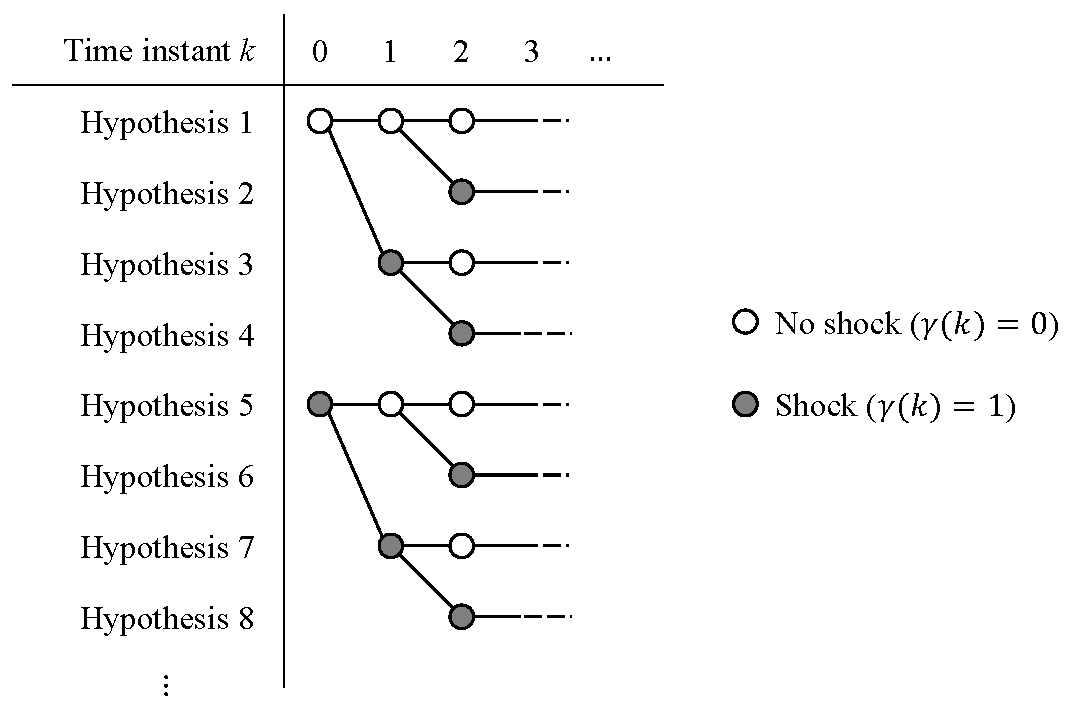
\includegraphics[height=7.5cm]{images/mm_obs_seq_br.pdf}
	\caption{Sequence branching}
	\label{fig:mm-obs-br}
\end{figure}


\subsubsection{Sequence fusion} \label{subsec-fusion}

\cite{robertson_detection_1995} propose a sub-optimal approach for RODD state estimation combining three approximations. The first is referred to as \textit{sequence fusion} or the \textit{generalized pseudo-Bayes algorithm} \citep{buxbaum_recursive_1969, jaffer_estimation_1971, tugnait_detection_1982}. This is based on the assumption that only recent differences in the shock hypothesis sequences are important for state estimation. Therefore, sequences which have the same values over the previous $f$ sample times, $\{\gamma(k-f+1), ...,  \gamma(k-1), \gamma(k)\}$, are combined. In other words, the maximum length of the unique sequences that must be modelled is $f$, which is known as the \textit{fusion horizon}. \textbf{TODO: $f$ clashes with use of $f$ as a filter index variable}

Secondly, they assume that the exact timing of the random shocks is not important and define \textit{detection intervals} of more than one sample period during which it is assumed that only one shock may occur. This is based on the observation that when the correction gain of a Kalman filter is increased, it tends to remain large for several sample periods. The probability of at least one random shock during a detection interval of length $d$ sample times is therefore
\begin{equation} \label{eq:p_gamma_d}
	\epsilon_d = 1 - (1 - \epsilon)^d.
\end{equation}

The probabilities of the modelled random shocks are then redefined as
\begin{equation} \label{eq:Pr_gamma_nd}
	\begin{aligned}
		\Pr\left(\gamma_{f}(k)=0\right) = \begin{cases*}
			1 - \epsilon_d & \text { for } $k = d, 2d, \ldots$ \\
			1 & \text { for } $k \ne d, 2d, \ldots$
		\end{cases*} \\
		\Pr\left(\gamma_{f}(k)=1\right) = \begin{cases*}
			\epsilon_d & \text { for } $k = d, 2d, \ldots$ \\
			0 & \text { for } $k \ne d, 2d, \ldots$
		\end{cases*} \\
	\end{aligned}
\end{equation}

Thirdly, they rely on the fact that the random shocks occur infrequently and therefore the probability that more than $m$ shocks occur during the fusion horizon is low, where $m$ may be 1 or a low number. This further reduces the number of filters required.

To illustrate this sequence fusion procedure, consider a simple example. Suppose there is one RODD to estimate and a sequence fusion algorithm is used with a detection interval of $d=3$ and a maximum number of shocks over the fusion horizon of $m=1$. Figure \ref{fig:mm-obs-seq-rob1} shows the four hypotheses that would be required in this case. Note that hypothesis 1 assumes no shocks at any time. Hypothesis 2 assumes shocks occur at times $k=0,9,18,...$. Hypothesis 3 assumes shocks occur at times $k=3,12,21,...$, and so on. After $f=9$ sample periods the sequences repeat indefinitely. 
\begin{figure}[htp]
	\centering
	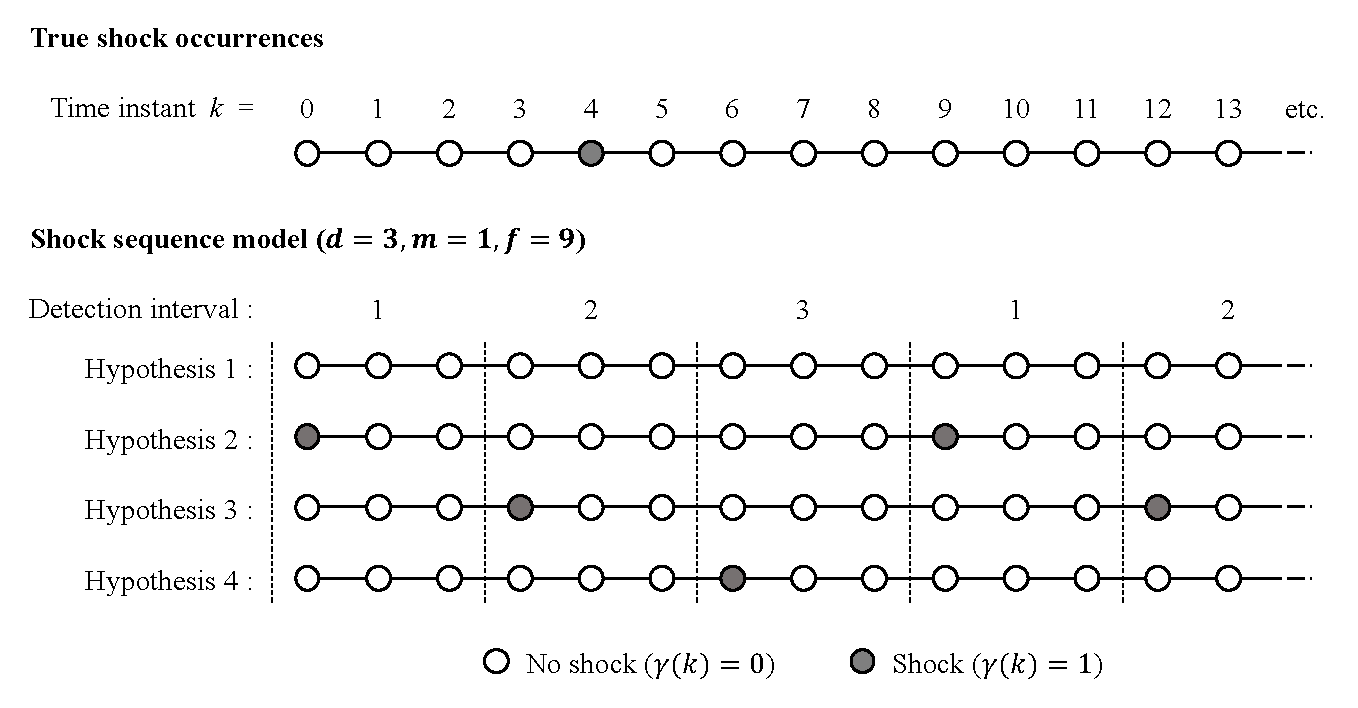
\includegraphics[height=5.3cm]{images/mm_obs_seq_rob1.pdf}
	\caption{Sequence fusion example 1 ($d=3$, $m=1$, $f=9$)}
	\label{fig:mm-obs-seq-rob1}
\end{figure}
If a shock actually occurred in the system at time $k=4$, for example, then the algorithm should estimate that hypothesis 3 is the most likely because this assumes a shock occurred at $k=3$, which is the close to reality.

Figure \ref{fig:mm-obs-seq-rob2} illustrates a second example of the sequence fusion algorithm with $m=2$ and a longer detection interval, $d=5$.  Note that this also has four hypotheses and that hypothesis 4 includes the case of two shocks within the fusion horizon. As in the previous example, if a true shock occurred at time $k=4$, the estimated most likely hypothesis should be hypothesis 3 because it assumes one shock occured at $k=5$, which is close to reality.

\begin{figure}[htp]
	\centering
	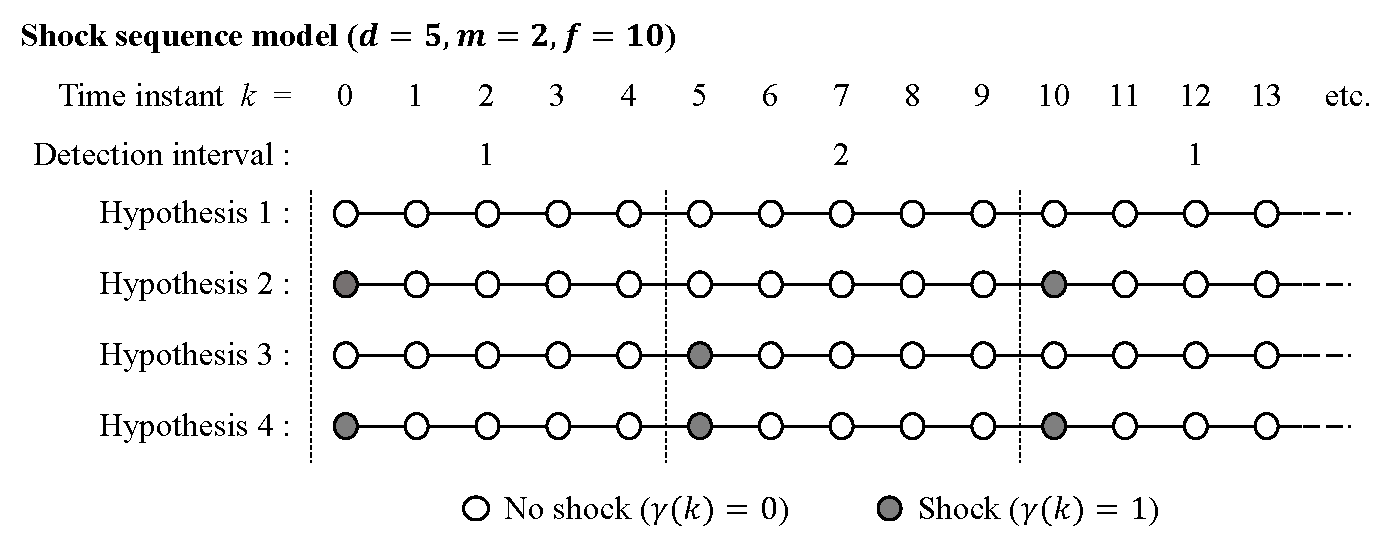
\includegraphics[height=5.3cm]{images/mm_obs_seq_rob2.pdf}
	\caption{Sequence fusion example 2 ($d=5$, $m=2$, $f=10$)}
	\label{fig:mm-obs-seq-rob2}
\end{figure}

\cite{robertson_detection_1995} describe a systematic procedure to choose the $f$, $d$, and $m$ parameters, and give the formula for the total probability of the modelled hypotheses up to time $k=nd$:
\begin{equation} \label{eq:p_gamma}
	\operatorname{Pr}\left(\sum_{i=1}^{n} \gamma(i d) \leq m\right) = \sum_{j=0}^{m} \binom{n}{j} \epsilon_p^{n-j}(1-\epsilon_p)^{j},
\end{equation}
where $\binom{n}{j}$ represents the number of possible combinations of $j$ shocks in $n$ intervals. They recommend that the total probability modelled should be at least 0.99 to ensure that only low-probability hypotheses are ignored.

In a later paper, \cite{robertson_method_1998} describe a variation to the sequence fusion algorithm described above.  Rather than assuming that the shock occurs in the first sample period of each detection interval, as shown in Figures \ref{fig:mm-obs-seq-rob1} and \ref{fig:mm-obs-seq-rob2}, they propose to represent the shock as a sequence of $d$ smaller shocks such that the total variance over the detection interval is the same as that of one shock. They claim that this improved the performance of the algorithm in simulations.

To implement this, first define a new variable to represent whether or not at least one shock occurs during the $n$\textsuperscript{th} detection interval:

\begin{equation} \label{eq:deltak}
	\delta(n) = \begin{cases*}
		0 & \text{if} $\sum_{k=(n-1) d}^{n d-1} \gamma_{k}=0$, \\
		1 & \text{if} $\sum_{k=(n-1) d}^{n d-1} \gamma_{k}\ge0$.
	\end{cases*}
\end{equation}

Then, replace the random shock variable used at each sample time, $w_p(k)$ (\ref{eq:wpk2}), with:
\begin{equation} \label{eq:wpdk}
	w_{p,d}(k) \sim 
	\begin{cases*}
		\mathcal{N}\left(0, \sigma_{w_p}^2\right) & \text{when} $\delta(n) = 0$, \\
		\mathcal{N}\left(0, \frac{b^2\sigma_{w_p}^2}{d}\right) & \text{when} $\delta(n) = 1$.
	\end{cases*}
\end{equation}

Note that the variance of a single shock, $b^2\sigma_{w_p}^2$, is divided by the interval length $d$.

\subsubsection{Sequence pruning} \label{subsec-pruning}

\textit{Sequence pruning} is the selective branching and deletion of shock hypotheses that have a low likelihood given the current measurements. The \textit{adaptive forgetting through multiple models} (AFMM) algorithm by \cite{andersson_adaptive_1985}, which was used by \cite{eriksson_classification_1996} for RODD estimation, uses sequence pruning to limit the number of filters required. In this algorithm, the current set of hypotheses are ranked at each time step, according to their conditional probabilities calculated using (\ref{eq:Pr_Gammak_given_Yk}). The hypothesis with the lowest probability is then pruned with the caveat explained below. The most probable hypothesis is allowed to branch but all other hypotheses are advanced assuming no shock occurs in the next time period (i.e. all but one of their branches are pruned). This makes sense in the case of RODD disturbances because the probability of a shock is low. Thus, the total number of hypotheses and filters is capped at a fixed number, $n_f$.

The caveat mentioned above, is that no hypothesis may be eliminated less than $n_{min}$ time steps after being created. This is to prevent good hypotheses from being eliminated before the conditional probabilities have been properly estimated, which can take more than one sample period. For this reason, $n_f$ must be at least sufficient to accommodate the \textit{minimum life}, $n_{min}$, of new hypotheses. Note that in the case of systems with more than one RODD disturbance, the number of branches of the most likely sequence is more than two, therefore a larger number of sequences will be pruned at each sample time.

To illustrate the sequence pruning procedure, consider the diagram in Figure \ref{fig:mm-obs-seq-erik}. This shows the possible evolution of the hypothesis sequences in response to an actual shock sequence consisting of one shock at time $k=4$.  The most likely hypotheses at each time instant, identified by the circles with thicker outlines, branch into two at the next time instant. After the limit of five hypotheses is reached, one hypothesis is pruned at each sample time and replaced by a new branched hypothesis at the next sample time. At time $k=6$, hypothesis 2 becomes the most likely based on the available measurements at that time. Also note that no new branches are terminated in less than two sample times.

\begin{figure}[htp]
	\centering
	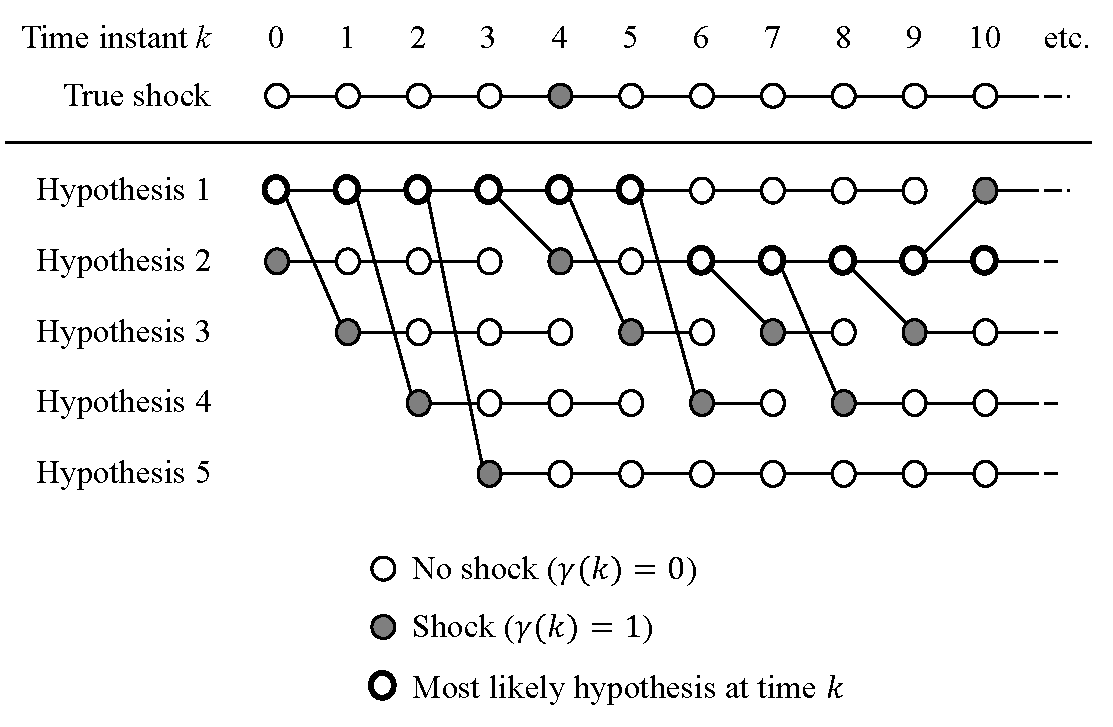
\includegraphics[height=7.5cm]{images/mm_obs_seq_erik.pdf}
	\caption{Sequence pruning example ($n_f=5$, $n_{min}=2$)}
	\label{fig:mm-obs-seq-erik}
\end{figure}

The AFMM algorithm by \cite{gustafsson_estimation_1993} includes a procedure for online estimation of the measurement noise covariance using a forgetting factor to control the speed of adaptation of the estimates. This component was not implemented in this work since it is assumed the measurement noise is time invariant.

\section{System identification}

Outline notes:
\begin{itemize}
	\item Explain Isaksson and Eriksson's perspective on standard system identification approach.
	\item Explain distinction between system detection or 'discrimination' and system identification, reference Isaksson and Eriksson's paper on disturbance classification (whether disturbance at input or output of process).
	\item Introduce other approaches—MLE, EM algorithm (Dempster et al., Wong \& Lee)
	\item Methods proposed by Bemporad (Fitting jump models, 2018 and Jump Box-Jenkins, 2020).
	\item Theory and challenges Costa book. Others?
	\item In recent years, numerical methods to overcome the intractability of the probabilistic integral have received a lot of attention.
	\item Sequential Monte-Carlo methods, (incl. particle filtering), Stochastic Variational Inference, ... (read Special issue in IEEE control magazine for an overview of these methods)
\end{itemize}

% Note: may remove this if we aren’t using any formal methods.

\section{Control strategies}

In this work, the goal is to test the performance of different observers in a closed-loop feedback control application (not to evaluate different control strategies). Therefore, only one control strategy is considered. According to the \textit{separation principle} of estimation and control, the control strategy may be designed independently of the observer. The controller is designed using the same model of the augmented system, including the plant model and disturbance models. However, the switching behaviour of the random shock variable used in the RODD is not explicitly considered in the control design. The estimates of the model states produced by the observer are assumed to be optimal, i.e. the expected values, and their uncertainty is not taken into account by the control algorithm or in its design.


\subsection{Model predictive control}

\textit{Model predictive control} (MPC) is a well known and widely used multi-variable control algorithm used in industrial applications. This is largely due to the fact that constraints can be imposed on the manipulatable variables and control variables, as well as its intuitive design and the ease with which it can be tuned to achieve control objectives \citep{maciejowski_predictive_2002}. Although it is a computationally complex algorithm, numerous proven commercial products exist to enable its implementation.

MPC utilizes a prediction equation based on the dynamic model of the system to find feasible future trajectories of the system outputs as a function of the manipulatable variables and the states of the model at the current. The length of the prediction horizon, $H_p$, is defined in terms of the number sample times starting at the next time instant, $k+1$. The predicted outputs over the prediction horizon, calculated at the current time $k$, are denoted $\hat{\textbf{y}}(k+i / k)$ for $i=1,2,...,H_p$. The length of the control horizon, $H_c$, is defined starting at the current time, $k$, and the manipulatable inputs are denoted $\mathbf{u}(k+i-1)$ for $i=1,2,...,H_c$. The control horizon is usually shorter than the prediction horizon, in which case, $\mathbf{u}(k+j)=\mathbf{u}(k+H_c-1)$ for $j=H_c,H_c+1,...,H_p$.

The constrained optimization problem, which is solved at each time step, is
\begin{align} \label{eq:mpc-opt}
	\begin{split}
		\min _{\mathbf{u}(k), \mathbf{u}(k+1), \ldots, \mathbf{u} (k+H_c-1)}
		& \quad \sum_{i=1}^{H_{p}}[\mathbf{\hat{y}}(k+i / k) - \mathbf{r}(k+i)]^\intercal \mathbf{\Phi} [\mathbf{\hat{y}}(k+i / k) - \mathbf{r}(k+i)] \\
		& \qquad + \sum_{i=1}^{H_{c}}[\Delta \mathbf{u}(k+i-1)]^\intercal \mathbf{\Lambda} [\Delta \mathbf{u}(k+i-1)] \\
			\end{split} \\
		\text { subject to: }
		&\ \mathbf{u}_{min} \leq \mathbf{u}(k+j-1) \leq \mathbf{u}_{max} \quad  j=1,2, \dots, H_{c} \label{eq:mpc-cons-1}, \\
		& \Delta \mathbf{u}_{min} \leq \Delta \mathbf{u}(k+j-1) \leq \Delta \mathbf{u}_{max} \quad j=1,2, \dots, H_{c}, \label{eq:mpc-cons-2} \\
		& \mathbf{y}_{min} \leq \mathbf{\hat{y}}(k+j / k) \leq \mathbf{y}_{max} \quad  j=1,2, \dots, H_{p}, \label{eq:mpc-cons-3}
\end{align}
where $\mathbf{r}(k+i)$ for $i=1,2,...,H_p$ is the reference output trajectory, and $\Delta \mathbf{u}(k)$ is the change in the manipulatable variable at time $k$, defined as $\Delta \mathbf{u}(k) = \mathbf{u}(k) - \mathbf{u}(k-1)$. The tunable parameters are $H_p$, $H_c$, $\mathbf{\Phi}$, and $\mathbf{\Lambda}$, and the constraints are $\mathbf{u}_{min}$, $\mathbf{u}_{max}$, $\Delta \mathbf{u}_{min}$, $\Delta \mathbf{u}_{max}$, $\mathbf{y}_{min}$, and $\mathbf{y}_{max}$. Note that the last constraint (\ref{eq:mpc-cons-3}) only guarantees that the estimate of the system output will not violate the constraints. This does not imply that the true system output will respect them at all times.

Once a solution to the optimization problem is found, only the control actions at the current time, $\mathbf{u}(k)$, are transmitted to the plant. The procedure is then repeated every future time instant to compute the subsequent control actions. This is referred to as a \textit{receding horizon control}.


\section{Grinding simulation model}

Outline notes:
\begin{outline}
    \1 Assumptions and limitations: constant breakage rate model, relationships between speed, media, trajectories, filling level and breakage not captured.
	\1 Describe grate, transport delays and cyclone model.
	\1 Outline any significant changes made from Edgar's model
	\1 Figure: simulation results showing steady-state characteristics - e.g. power, grind, and throughput vs. fill level and speed.
	\1 Figure \ref{fig:coarse_fine_psd_plot}: Particle size distributions of feed, recirculating load and product - this should help explain steady-state characteristics.
	\1 Figure - Step responses of main process variables to changes in ore properties.
	\1 Selection of particle size distribution as the disturbance variable for this work.
	\1 Steady-state characteristics with operating points (grind curves)\\
\end{outline}


A dynamic simulation model of the primary grinding circuit of a gold mine in Quebec is used to simulate the effects of changes in ore feed properties over time. The model was developed by \cite{perez_garcia_dynamic_2020} following the methodology described by \cite{grimble_dynamic_2010} and was calibrated to match the operating data from the real plant \citep{perez-garcia_systematic_2020}. The SAG mill component is a \textit{population balance model} with 24 discrete size intervals for ore particles with constant specific-energy selection rates (i.e. breakage rates are proportional to total energy consumption) and a constant breakage matrix.

Figure \ref{fig:sag-diag} is a simplified diagram of the simulated circuit, consisting of a feed conveyor, SAG mill, pump box, pump, and a bank of hydro-cyclones.
\begin{figure}[htp]
	\centering
	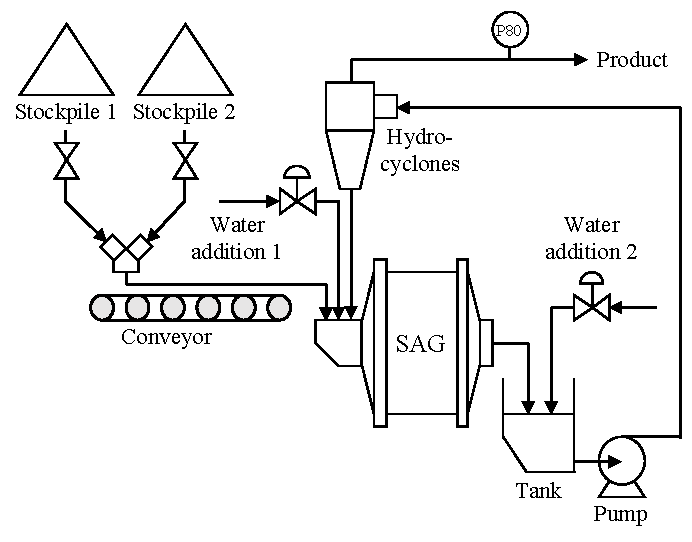
\includegraphics[width=11cm]{images/sag-circuit-diag.pdf}
	\caption{Simplified process flow diagram}
	\label{fig:sag-diag}
\end{figure}
For the purposes of this work, two ore streams with different PSDs were configured to feed the circuit. Each stream is a different mix of two different ores. One ore has a fine PSD and the other is coarse. The mix for stream \#1 (`mix 1') consists of 22.83\% coarse ore (\textit{mix factor} of 0.2283) and mix \#2 is an even mix of both ores (mix factor of 0.5). Figure \ref{fig:coarse_fine_psd_plot} shows the PSDs of the two ore sources and the two mixtures.

\begin{figure}[htp]
	\centering
	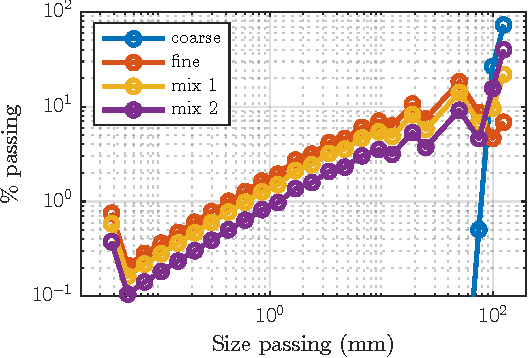
\includegraphics[width=9cm]{images/coarse_fine_psd_plot.pdf}
	\caption{Ore particle size distributions}
	\label{fig:coarse_fine_psd_plot}
\end{figure}

The SAG mill water addition set-point is set by ratio control to a ratio of the fresh ore feed rate. This ratio may be manipulated by the control system. The pump-box level has a PI (proportional-integral) controller to control the level to a fixed set-point by manipulating the water addition rate set-point. The discharge pump speed is fixed. Conveyor speed is adjusted automatically in response to the fresh ore feed rate. Total ore feed rate and the SAG rotational speed set-point may also be manipulated by a control system.

The main measurable process variables are mill weight, power consumption, circulating load flow rate, and the solids-content (\%) of the cyclone feed. The P80 (80\% passing size) of the ground product leaving the cyclone overflow is also measured. Mill filling level and many other simulation variables are available for analysis but are assumed to be unmeasured in the real operation and therefore not available for process control.

Zero-mean Gaussian measurement noises are added to the output variables to simulate measurement errors. The parameters for these noises and other information on all the process variables are shown in Table X. Except for the measurement noises and the input disturbances described in subsequent sections, the model itself is deterministic.

%TODO: Table of process variables and normal operating points, limits etc.

Although some of these process variables would likely be sampled at higher rates in practice, it is assumed, for simplicity, that they are all sampled at the same rate of 1 sample every 3 minutes (i.e. a sampling period of 0.05 hours). This was deemed to be a typical sampling rate of a standard online particle size analyser that would be used for the P80 measurement.


\section{Performance evaluation}

Outline notes:
\begin{itemize}
	\item Comparing disturbance state estimate to true disturbance (simulation only).
	\item Tracking error: Mean-squared difference of output estimates. (or use RMSE?)
	\item Partitioning of simulation outputs into 'transition periods' and steady-state periods.
	\item Variance of output estimate in steady-state (no disturbances).
	\item Mean-squared differences in estimates (similar to variance but with no bias).
	\item Sensitivity to model errors, observer parameters.
	\item Closed loop stability - stability margins.
\end{itemize}

